\documentclass[a4paper,titlepage]{report}

%PACKAGES
\usepackage[utf8]{inputenc}
\usepackage[T1]{fontenc}
\usepackage[francais]{babel}
\usepackage{amsmath}
\usepackage{amssymb}
\usepackage{mathrsfs}
\usepackage{fancyhdr}
\usepackage{lmodern}
\usepackage{graphicx}
\usepackage{geometry}
\usepackage{fancybox}
\usepackage{textcomp}
\usepackage{subfigure}

%Symbole euro
\usepackage{eurosym}

%Listings : affichage code
\usepackage{listings}


%Elements de la page de garde
\begin{document}

\begin{titlepage}

\begin{figure}
\centering

\includegraphics[width=5cm]{logo-ulg.png}
\end{figure}



\title{
\vspace{0.2cm}
\LARGE{\textbf{Projet 1 - Chaînes de Markov}} \\ \textsc{Eléments de processus stochastiques}
\author{\textbf{Floriane Magera} \\ \textbf{Romain Mormont} \\ \textbf{Fabrice Servais}\\ Troisième bachelier en sciences de l'ingénieur}
\date{}
\rule{15cm}{1.5pt}
}

%\geometry{hmargin=2.5cm}
\end{titlepage}

%DOCUMENT
\pagestyle{fancy}
\lhead{Projet 1 - Chaînes de Markov}
\rhead{Éléments de processus stochastiques}

%Page de garde
\maketitle

\newpage
\section{Question 1.2 : téléportation}
\paragraph{1)}
La formule utilisée pour calculer la matrice de transition $Q_t$ du modèle du surfeur avec téléportation est la suivante :
\[
	Q_t = (1 - \alpha) Q' + \alpha \tilde{Q}
\]
où $Q'$ et $\tilde{Q}$ sont des matrices de transition et $\alpha$ la probabilité de téléportation. 
\paragraph{}
La première est la matrice de transition du graphe initial auquel on a rajouté des arêtes partant des \textit{dangling nodes}. Elle a été calculée en remplaçant tous les éléments de la matrice $Q$ dans des lignes ne contenant que des 0 par $\frac{1}{n}$. Cette valeur $\frac{1}{n}$ a été choisie en considérant une densité de probabilité uniforme entre les différentes arêtes partant des \textit{dangling nodes}. 
\paragraph{}
La seconde est la matrice de transition du graphe complet formé des noeuds du graphe initial. Autrement dit, la matrice de transition représentant la téléportation. Une combinaison linéaire de paramètre $\alpha$ est ensuite appliquée aux deux matrices pour trouver la matrice $Q_t$.
\paragraph{2)}
Pour que la distribution stationnaire $\pi_s$ soit unique, \textbf{il faut que la chaîne de Markov soit irréductible}. Autrement dit, il faut que pour tout couple de nœuds $(i_1$, $i_2)$, il existe une arête les reliant (un probabilité non-nulle de passer de $i_1$ à $i_2$). Cette propriété est vérifiée avec le modèle du surfeur modifié puisque la téléportation permet, depuis tout noeud, de se diriger vers un autre noeud tant que $\alpha > 0$. 
\paragraph{}
A partir du moment où $\alpha = 0$, on est plus assuré que chaque paire de nœuds est reliée par une arête et donc que $\pi_s$ est bien stationnaire.
\paragraph{3)} 
Les sites les plus visités, obtenus à l'aide de la distribution stationnaire, sont les suivants :
\begin{enumerate}
	\item http://purl.org/rss/1.0/modules/content
    \item http://www.ulg.ac.be
    \item http://ogp.me/ns$\sharp$
    \item http://www.gre-liege.be
    \item http://blog.intelliterwal.net
    \item http://www.jalios.com
    \item http://www.vmfnet.be
    \item http://www.alinoa.be
    \item http://www.ulb.ac.be
    \item http://www.cedia.ulg.ac.be
\end{enumerate}
\paragraph{4)}
\section{Question 1.3 : effet de $\alpha$}
\paragraph{1)}
Pour prouver que le score PageRank de toute page est au moins $\frac{\alpha}{n}$ ($n$ est le nombre de pages), on peut développer une expression "\textit{explicite}" des éléments de la matrice $Q_t$ en utilisant la formule donnée précédemment : 
\[
\begin{aligned}
Q_t(i,j) = q_{ij} (1 - \alpha) + \dfrac{1}{n}\alpha\\
\end{aligned}
\]
où $q_{ij}$ est un élément de la matrice $Q'$. Connaissant la relation qui lie $\pi^{(k)}$ et $\pi^{(k-1)}$, on a :
\[
\begin{aligned}
\pi^{(k)}_j &= \sum\limits_{i = 1}^n Q_t(i,j)\pi^{(k-1)}_j\\
 &= \sum\limits_{i = 1}^n \left(q_{ij} (1 - \alpha) + \dfrac{\alpha}{n}\right)\pi^{(k-1)}_j\\
 &= \sum\limits_{i = 1}^n q_{ij} (1 - \alpha) \pi^{(k-1)}_j + \sum\limits_{i = 1}^n \dfrac{\alpha}{n} \pi^{(k-1)}_j\\
 &= \dfrac{\alpha}{n} + \underbrace{(1 - \alpha) \sum\limits_{i = 1}^n q_{ij} \pi^{(k-1)}_j}_{> 0}
\end{aligned}
\]
Le deuxième terme est inférieur à 1 (et même inférieur à $(1 - \frac{\alpha}{n})$ afin de respecter le deuxième axiome de Kolmogorov) et surtout, positif. De ce fait, on peut affirmer que :
\[
\pi^{(k)}_j \geq \dfrac{\alpha}{n}
\]
\paragraph{}
Le cas où $\alpha$ tend vers 1 correspond à la situation où le surfeur a majoritairement tendance à se téléporter lorsqu'il change de page. Si on considère qu'en cas de téléportation, la distribution de probabilité est uniforme entre les nœuds de destination, on observera un PageRank uniforme. 
\paragraph{}
Afin de vérifier cette conclusion, nous avons calculé la distribution stationnaire pour un $\alpha = 1$. Le résulat est donné sur la Figure \ref{fig:q131_alpha} où il est mis en parallèle avec la distribution des pour $\alpha = 0.15$. Le résultat est édifiant, on constate en effet un PageRank uniforme dans le cas où $\alpha = 1$ (écart-type du PageRank: $4.7753\times 10^{-18}$).
\begin{figure}[h]
	\center
	\subfigure[{$\alpha = 0.15$}]{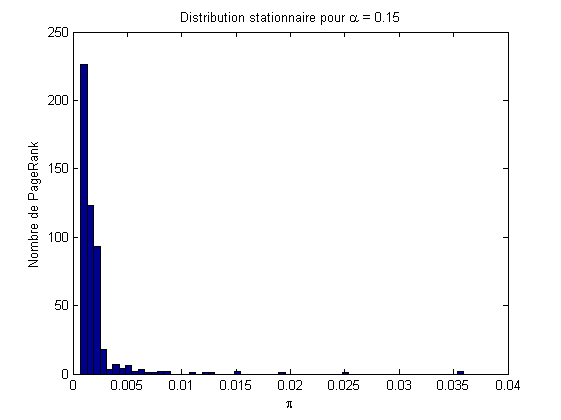
\includegraphics[scale=0.45]{q131_alpha015.png}}
	\subfigure[{$\alpha = 1$}]{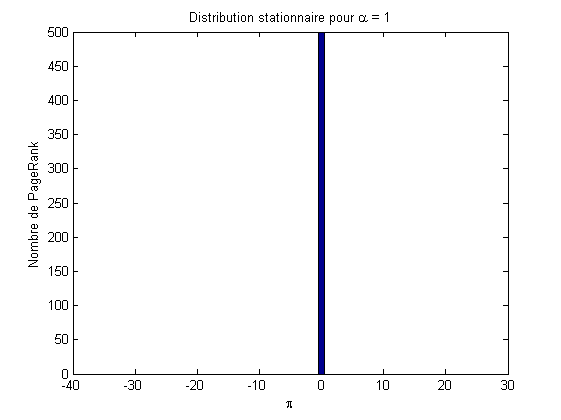
\includegraphics[scale=0.45]{q131_alpha1.png}}
	\caption{Distribution des PageRank lorsque $\alpha$ tend vers 1}
	\label{fig:q131_alpha}
\end{figure}
\end{document}